\documentclass[10pt,letterpaper]{article}

%\usepackage{cogsci}
\usepackage{pslatex}
\usepackage{apacite}
\usepackage{color}
\usepackage{amsmath}
\usepackage{amsfonts}
\usepackage{amssymb}
%\usepackage{widetext}
\usepackage{graphicx, caption, subcaption}
% subfig
\usepackage{fixltx2e}

% for leabra symbols
%
% General Text
%
%\newcommand{\vs}{{\em vs\/} }
%
% General Math
%
\newcommand{\avg}[1]{\overline{#1}}
\newcommand{\ev}[1]{\left<#1\right>}
\newcommand{\bvec}[1]{{\bf #1}}
%\newcommand{\ovavg}[2]{\stackrel{{\tiny #1}}{\overline{#2}}}
\newcommand{\ovavg}[2]{\langle #2 \rangle^{#1}}
\newcommand{\dxdy}[2]{\frac{d#1}{d#2}}
\newcommand{\pdxdy}[2]{\frac{\partial #1}{\partial #2}}
\newcommand{\pdxdysq}[2]{\frac{\partial^2 #1}{\partial^2 #2}}
\newcommand{\bico}[2]{\left( \begin{array}{c} #1 \\ #2 \end{array} \right)}
\newcommand{\aoverb}[2]{\begin{array}{c} #1 \\ #2 \end{array}}
\newcommand{\matonetwo}[2]{\left[ \begin{array}{c} #1 \\ #2 \end{array} \right]}
\newcommand{\matonethr}[3]{\left[ \begin{array}{c} #1 \\ #2 \\ #3 \end{array} \right]}
\newcommand{\mattwotwo}[4]{\left[ \begin{array}{cc}
    #1 & #2 \\ #3 & #4 \end{array} \right]}
\newcommand{\mattwothr}[6]{\left[ \begin{array}{cc}
    #1 & #2 \\ #3 & #4 \\ #5 & #6 \end{array} \right]}
\newcommand{\matthrtwo}[6]{\left[ \begin{array}{ccc}
    #1 & #2 & #3 \\ #4 & #5 & #6 \end{array} \right]}
\newcommand{\matthrthr}[9]{\left[ \begin{array}{ccc}
    #1 & #2 & #3 \\ #4 & #5 & #6 \\ #7 & #8 & #9 \end{array} \right]}
\newcommand{\diverge}[2]{#1\log\frac{#1}{#2} + (1-#1)\log\frac{1-#1}{1-#2}}
%
% Neural Network Symbols
%
\newcommand{\wij}{w_{ij}}
\newcommand{\wji}{w_{ji}}
\newcommand{\wjk}{w_{jk}}
\newcommand{\wkj}{w_{kj}}
\newcommand{\oneo}[1]{\frac{1}{#1}}
\newcommand{\Inet}{I^{net}}

\newcommand{\eqla}{\breve{a}}
\newcommand{\eqlG}{\breve{G}}
\newcommand{\eqlS}{\breve{S}}
\newcommand{\eqlH}{\breve{H}}
\newcommand{\eqlnet}{\breve{net}}
%
% Network Variables
%
\newcommand{\ai}{a_i}
\newcommand{\aj}{a_j}
\newcommand{\wnet}{w^{net}}
\newcommand{\wpre}{w^{pre}}
\newcommand{\wpost}{w^{post}}
%
% Bio Symbols
%
\newcommand{\Ca}{Ca^{2+}}
\newcommand{\Na}{Na^+}
\newcommand{\K}{K^+}
\newcommand{\Cl}{Cl^-}
\newcommand{\Mg}{Mg^{2+}}
\newcommand{\PrjTo}{\ensuremath{\Rightarrow}}
\newcommand{\PrjToFm}{\ensuremath{\Leftrightarrow}}
%
% Stats Symbols
%
\newcommand{\smean}{\overline{X}}
\newcommand{\sdiff}{s_{(\smean_A - \smean_B)}}
\newcommand{\spooled}{s_{pooled}}
\newcommand{\sems}{s_{\smean}}
\newcommand{\sem}{\sigma_{\smean}}
\newcommand{\dmean}{\overline{D}}
\newcommand{\semd}{s_{\dmean}}

%% END MACROS SECTION

\numberwithin{equation}{section}

\title{A continuous time neural model for sequential action: Supplemental Information}

\author{George Kachergis$^1$, Dean Wyatte$^2$, Randall C. O'Reilly$^2$, \\
	Roy de Kleijn$^1$, and Bernhard Hommel$^1$ \\
	\bf george.kachergis@gmail.com \\
	$^1$ Institute for Psychological Research \& \\
	Leiden Institute for Brain and Cognition, Leiden University \\
	$^2$ Department of Psychology and Neuroscience, \\
	University of Colorado Boulder }

\date{}

\begin{document}
\maketitle


%%%%%%%%%%%%%%%%%%%%%%%%%%%%%%%%%%%%%%%%%

\sloppy

% trim down xcal, integrate with TI section
% edit intro to foreshadow
% also note stable weights

\section{Leabra and LeabraTI: Implementation Details}

The Leabra framework is described in detail in \citeA{OReilly:2000,OReilly:book} and
\citeA{OReilly:2001}, and summarized here. The standard Leabra equations have been used to simulate over 40 different models in
\citeA{OReilly:2000} and a number of other research models. Thus, the
model can be viewed as an instantiation of a systematic modeling framework
using standardized mechanisms, instead of constructing new mechanisms for each
model.

This version of Leabra contains an extension called LeabraTI (Temporal Integration) that allows learning to operate over temporally contiguous input sequences. 
The full treatment of LeabraTI is presented in an in-preparation paper \cite{OReilly:LeabraTI}, but the basic equations and a brief motivation for them are
presented here.

\subsection{Point Neuron Activation Function} 

Leabra uses a {\em point neuron} activation function that models the
electrophysiological properties of real neurons, while simplifying their
geometry to a single point. This function is nearly as simple computationally
as the standard sigmoidal activation function, but the more biologically-based
implementation makes it considerably easier to model inhibitory competition,
as described below. Further, using this function enables cognitive models to
be more easily related to more physiologically detailed simulations, thereby
facilitating bridge-building between biology and cognition. We use normalized
units where the unit of time is 1 msec, the unit of electrical potential is
0.1 V (with an offset of -0.1 for membrane potentials and related terms, such
that their normal range stays within the $[0, 1]$ normalized bounds), and the unit
of current is $1.0x10^{-8}$.

The membrane potential $V_m$ is updated as a function of ionic
conductances $g$ with reversal (driving) potentials $E$ as follows:
\begin{equation}
 \Delta V_m(t) = \tau \sum_c g_c(t) \overline{g_c} (E_c - V_m(t))
 \label{eq.vm}
\end{equation}
with 3 channels ($c$) corresponding to: $e$ excitatory input; $l$ leak
current; and $i$ inhibitory input. Following electrophysiological
convention, the overall conductance is decomposed into a time-varying
component $g_c(t)$ computed as a function of the dynamic state of the
network, and a constant $\overline{g_c}$ that controls the relative
influence of the different conductances. The equilibrium potential
can be written in a simplified form by setting the excitatory driving
potential ($E_e$) to 1 and the leak and inhibitory driving potentials
($E_l$ and $E_i$) of 0:
\begin{equation}
 V_m^\infty = \frac{g_e \overline{g_e}} {g_e
  \overline{g_e} + g_l \overline{g_l} + g_i \overline{g_i}} 
\end{equation}
which shows that the neuron is computing a balance between excitation
and the opposing forces of leak and inhibition. This equilibrium form
of the equation can be understood in terms of a Bayesian decision
making framework \cite{OReilly:2000}.

The excitatory net input/conductance $g_e(t)$ or $\eta_j$ is computed
as the proportion of open excitatory channels as a function of sending
activations times the weight values:
\begin{equation}
 \eta_j = g_e(t) = \langle x_i \wij \rangle = \oneo{n} \sum_i x_i \wij
 \label{eq.net_in_avg}
\end{equation}
The inhibitory conductance is computed via the kWTA function described
in the next section, and leak is a constant.

In its discrete spiking mode, Leabra implements exactly the AdEx (adaptive
exponential) model \cite{Brette:2005}, which has been found through
various competitions to provide an excellent fit to the actual firing
properties of cortical pyramidal neurons \cite{Gerstner:2009}, while
remaining simple and efficient to implement. However, we typically use a
rate-code approximation to discrete firing, which produces smoother more
deterministic activation dynamics, while capturing the overall firing rate
behavior of the discrete spiking model.

We recently discovered that our previous strategy of computing a rate-code
graded activation value directly from the membrane potential is problematic,
because the mapping between $V_m$ and mean firing rate is not a one-to-one
function in the AdEx model. Instead, we have found that a very accurate
approximation to the discrete spiking rate can be obtained by comparing the
excitatory net input directly with the effective computed amount of net input
required to get the neuron firing over threshold ($g_e^{\Theta}$), where the
threshold is indicated by $\Theta$:
\begin{equation}
g_e^{\Theta} = \frac{g_i \overline{g}_i (E_i - V_m^{\Theta}) +
 \overline{g}_l(E_l - V_m^{\Theta})} {\overline{g}_e (V_m^{\Theta} - E_e)}
\end{equation}
\begin{equation}
 y_j(t) \propto g_e(t) - g_e^{\Theta}
\end{equation}
where $y_j(t)$ is the firing rate output of the unit.

We continue to use the Noisy X-over-X-plus-1 (NXX1) function, which starts out
with a nearly linear function, followed by a saturating nonlinearity:
\begin{equation}
 y_j(t) = \oneo{\left(1 + \oneo{\gamma [g_e(t) - g_e^{\Theta}]_+} \right)}
\end{equation}
where $\gamma$ is a gain parameter, and $[x]_+$ is a threshold function that
returns 0 if $x<0$ and $x$ if $x>0$. Note that if it returns 0, we assume
$y_j(t) = 0$, to avoid dividing by 0. As it is, this function has a very
sharp threshold, which interferes with graded learning learning mechanisms
(e.g., gradient descent). To produce a less discontinuous deterministic
function with a softer threshold, the function is convolved with a Gaussian
noise kernel ($\mu=0$, $\sigma=.005$), which reflects the intrinsic processing
noise of biological neurons:
\begin{equation}
 y^*_j(x) = \int_{-\infty}^{\infty} \oneo{\sqrt{2 \pi} \sigma}
 e^{-z^2/(2 \sigma^2)} y_j(z-x) dz
 \label{eq.conv}
\end{equation}
where $x$ represents the $[g_e(t) - g_e^{\Theta}]_+$ value, and $y^*_j(x)$
is the noise-convolved activation for that value. In the simulation,
this function is implemented using a numerical lookup table.

\subsection{k-Winners-Take-All Inhibition}

Leabra uses a kWTA (k-Winners-Take-All) function to achieve inhibitory
competition among units within a layer (area). The kWTA function
computes a uniform level of inhibitory current for all units in the
layer, such that the $k+1$th most excited unit within a layer is
generally below its firing threshold, while the $k$th is typically
above threshold. Activation dynamics similar to those produced by the
kWTA function have been shown to result from simulated inhibitory
interneurons that project both feedforward and feedback inhibition
\cite{OReilly:2000}. Thus, although the kWTA function is
somewhat biologically implausible in its implementation (e.g.,
requiring global information about activation states and using sorting
mechanisms), it provides a computationally effective approximation to
biologically plausible inhibitory dynamics.

kWTA is computed via a uniform level of inhibitory current for all
units in the layer as follows:
\begin{equation}
 g_i = g^{\Theta}_{k+1} + q (g^{\Theta}_k - g^{\Theta}_{k+1})
 \label{eq.g_i}
\end{equation}
where $0<q<1$ (.25 default used here) is a parameter for setting the
inhibition between the upper bound of $g^{\Theta}_k$ and the lower
bound of $g^{\Theta}_{k+1}$. These boundary inhibition values are
computed as a function of the level of inhibition necessary to keep a
unit right at threshold $\Theta$:
\begin{equation}
 g_i^{\Theta} = \frac{g^*_e \bar{g_e} (E_e - \Theta) +
  g_l \bar{g_l} (E_l - \Theta)}{\Theta - E_i}
 \label{eq.i_at_thr}
\end{equation}
where $g^*_e$ is the excitatory net input without the bias weight
contribution --- this allows the bias weights to override the kWTA
constraint.

In the basic version of the kWTA function, which is relatively rigid
about the kWTA constraint and is therefore used for output layers,
$g^{\Theta}_k$ and $g^{\Theta}_{k+1}$ are set to the threshold
inhibition value for the $k$th and $k+1$th most excited units,
respectively. Thus, the inhibition is placed exactly to allow $k$
units to be above threshold, and the remainder below threshold. For
this version, the $q$ parameter is almost always .25, allowing the
$k$th unit to be sufficiently above the inhibitory threshold.

In the {\em average-based} kWTA version, $g^{\Theta}_k$ is the average
$g_i^{\Theta}$ value for the top $k$ most excited units, and
$g^{\Theta}_{k+1}$ is the average of $g_i^{\Theta}$ for the remaining
$n-k$ units. This version allows for more flexibility in the actual
number of units active depending on the nature of the activation
distribution in the layer and the value of the $q$ parameter (which is
typically .6), and is therefore used for hidden layers.

\subsection{Learning rules} 

The model uses both Leabra learning using the XCAL formulation (see \citeNP{OReillyWyatte:2013} Supplemental Information) as well as an extension called LeabraTI on specific projections.

\subsubsection{Leabra XCAL}

In Leabra XCAL, the error-driven and self-organizing factors emerge out of a
single learning rule based on a contrast between a sender-receiver
activation product term at three time scales:

\begin{itemize}
\item {\bf s} = short time scale, reflecting the most recent state of neural
 activity (e.g., past 100-200 msec). This is considered the ``plus phase''
 -- it represents the {\em outcome} information on the current trial, and in
 general should be more correct than the medium time scale.
\item {\bf m} = medium time scale, which integrates over an entire
 psychological ``trial'' of roughly a second or so -- this value contains a
 mixture of the ``minus phase'' and the ``plus phase'', but in contrasting it
 with the short value, it plays the role of the minus phase value, or
 expectation about what the system thought should have happened on the
 current trial.
\item {\bf l} = long time scale, which integrates over hours to days of
 processing -- this is a threshold term similar to that used in the  Bienenstock, Cooper \& Munro (BCM) algorithm \cite{Bienenstock:1982}.
\end{itemize}

The error-driven aspect of XCAL learning is driven essentially by the
following term: 
\begin{equation}
 \Delta_{xcal-err} \wij = f_{xcal} ( x_s y_s, x_m y_m )
 \label{eq.xcal-err}
\end{equation}
However, consider the case where either of the short term values ($x_s$ or
$y_s$) is 0, while both of the medium-term values are $>0$ -- from an
error-driven learning perspective, this should result in a significant weight
decrease, but because the XCAL function goes back to 0 when the input drive
term is 0, the result is no weight change at all. To remedy this situation,
we assume that the short-term value actually retains a small trace of the
medium-term value:
\begin{equation}
 \Delta_{xcal-err} \wij = f_{xcal} ( \kappa x_s y_s + (1-\kappa) x_m y_m, x_m y_m)
 \label{eq.xcal-err2}
\end{equation}
(where $\kappa = .9$, such that only .1 of the medium-term averages are
incorporated into the effective short-term average).

The self-organizing aspect of XCAL is driven by comparing this same synaptic
drive term to a longer-term average, as in the BCM algorithm:
\begin{equation}
 \Delta_{xcal-so} \wij = f_{xcal} ( \kappa x_s y_s + (1-\kappa) x_m y_m, \gamma_l y_l)
 \label{eq.xcal-selforg}
\end{equation}
where $\gamma_l = 3$ is a constant that scales the long-term average threshold
term (due to sparse activation levels, these long-term averages tend to be
rather low, so the larger gain multiplier is necessary to make this term
relevant whenever the units actually are active and adapting their weights).

Combining both of these forms of learning in the full XCAL learning rule
amounts to computing an aggregate $\theta_p$ threshold that reflects a
combination of both the self-organizing long-term average, and the medium-term
minus-phase like average:
\begin{equation}
 \Delta_{xcal} \wij = f_{xcal} ( \kappa x_s y_s + (1-\kappa) x_m y_m, \lambda
 \gamma y_l + (1-\lambda) x_m y_m)
 \label{eq.xcal}
\end{equation}
where $\lambda = .01$ is a weighting factor determining the mixture of
self-organizing and error-driven learning influences (as was the case with
standard Leabra, the balance of error-driven and self-organizing is heavily
weighted toward error driven, because error-gradients are often quite weak in
comparison with local statistical information that the self-organizing system
encodes).

The weight changes are subject to a soft-weight bounding to keep within the $0-1$
range:
\begin{equation}
 \Delta_{sb} \wij = [\Delta_{xcal}]_+ (1-\wij) + [\Delta_{xcal}]_- \wij
 \label{eq.err_soft_bound}
\end{equation}
where the $[]_+$ and $[]_-$ operators extract positive values or
negative-values (respectively), otherwise 0.

Finally, as in the original Leabra model, the weights are subject to contrast
enhancement, which magnifies the stronger weights and shrinks the smaller ones
in a parametric, continuous fashion. This contrast enhancement is achieved by
passing the linear weight values computed by the learning rule through a
sigmoidal nonlinearity of the following form:
\begin{equation}
 \hat{w}_{ij} = \oneo{1 + \left(\frac{\wij}{\theta (1-\wij)}\right)^{-\gamma}}
 \label{eq.wt_off}
\end{equation}
where $\hat{w}_{ij}$ is the contrast-enhanced weight value, and the
sigmoidal function is parameterized by an offset $\theta$ and a gain
$\gamma$ (standard defaults of 1 and 6, respectively, used here). 

\subsubsection{LeabraTI}
LeabraTI extends standard Leabra learning by interleaving its minus and plus phases over temporally contiguous input sequences. In standard Leabra, the minus phase depends on clamped inputs from the sensory periphery to drive the expectation while the plus phase uses clamped outputs from other neural systems to drive the outcome. In LeabraTI, the minus phase expectation is not driven by the sensory periphery, but instead by lagged context represented by deep (Layer 6) neurons. During the plus phase, driving potential shifts back to the sensory periphery. Deep neurons' context is also updated after each plus phase.

LeabraTI was only used to update the synaptic weights between superficial and deep neurons. Inter-areal feedforward and feedback projections bifurcate from the local column, directly synapsing disparate populations of superficial neurons and thus weight updates in these cases were handled by Leabra XCAL equations. In computing the weight update, the standard Leabra delta rule \cite{OReilly:1996} uses the difference in rate between the plus and minus phases of receiving units (\textit{y}) in proportion to the rate of sending units (\textit{x}) in the minus phase:
\begin{align*}
\Delta_{leabra} w_{ij} &= x^-(y^+ - y^-)
\end{align*}

In the LeabraTI framework, deep neurons are considered to be the receiving units as they are the terminus of the descending columnar synapses. However, deep units are proposed to only be active during the minus phase when they drive the prediction, and thus cannot be used to compute an error signal.  To address this issue, we invert the LeabraTI delta rule:
\begin{align*}
\Delta_{leabrati} w_{ij} &= super^-(deep^+ - deep^-) \\
			  &\approx deep^-(super^+ - super^-)
\end{align*}

Additionally, the temporally extended nature of the algorithm requires that the receiving units represent the current state (time \textit{t}) and sending units the previous moment's state (time \textit{t} - 1). While conceptualized as the previous equation, the actual implementation is as follows:
\begin{align*}
\Delta_{leabrati} w_{ij} &= super_{t-1}^+(super_{t}^+ - super_{t}^-)
\end{align*}

This formulation allows the driving potential of deep neurons to be computed just once using the previous plus phase state of superficial neurons (multiplied by the superficial $\rightarrow$ deep learned weights) and held constant as an input to superficial neurons during the minus phase. This is a gross simplification of the actual biological process of deep neurons, but is vastly more computationally efficient than explicit modeling by computing an additional rate for each deep neuron at each time step. This formulation is also equivalent to the simple recurrent network (SRN) \cite{Elman:1990,Servan-Schreiber:1991}, thus providing a potential biological substrate for its computational function. 

One limitation of LeabraTI's interleaving of minus and plus phases over time is that the initial minus phase in an input sequence does not have access to the previous moment's  context. Even if there was lagged context available, it would represent information from a prior, possibly unrelated input sequence. To address this, weight updates are disabled for the first minus-plus phase pair, and enabled thereafter. In the brain, this process might be facilitated by a neural mechanism that is sensitive to the repetition of inputs over time (e.g., acetylcholine) \cite{Thiel:2001,Thiel:2002}.


\section{Training Details}

[Detailed description of CoffeeTeaEnv from Randy?]

Using 2 hidden layers with 24 units each, 100 networks were trained over 200 50-step epochs. The learning rate was 0.5 until epoch 50, dropping to 0.2 until epoch 100, then dropped to 0.1 until epoch 150, and finally dropped to 0.05 for the final 50 epochs. Training accuracy for the final 50 epochs was 94\% for the model with 2 24-unit hidden layers, and 95\% for the single 48-unit hidden layer model. Normalized error was .016 for the two layer model, compared to .017 for the single layer model.

\section{Test Results}

Shown in Figure~\ref{fig:test_error}, the normal network weights perform very well for almost all test trials, whereas the Non-TI version performs very poorly for nearly all trials. Lesioning the second hidden layer (Hid2 Lesion) impacted performance somewhat, and more for some steps than others. Weakening the context projections had a larger impact on performance, but were still much better than the Non-TI network.

\begin{figure}[h]
  \centering
  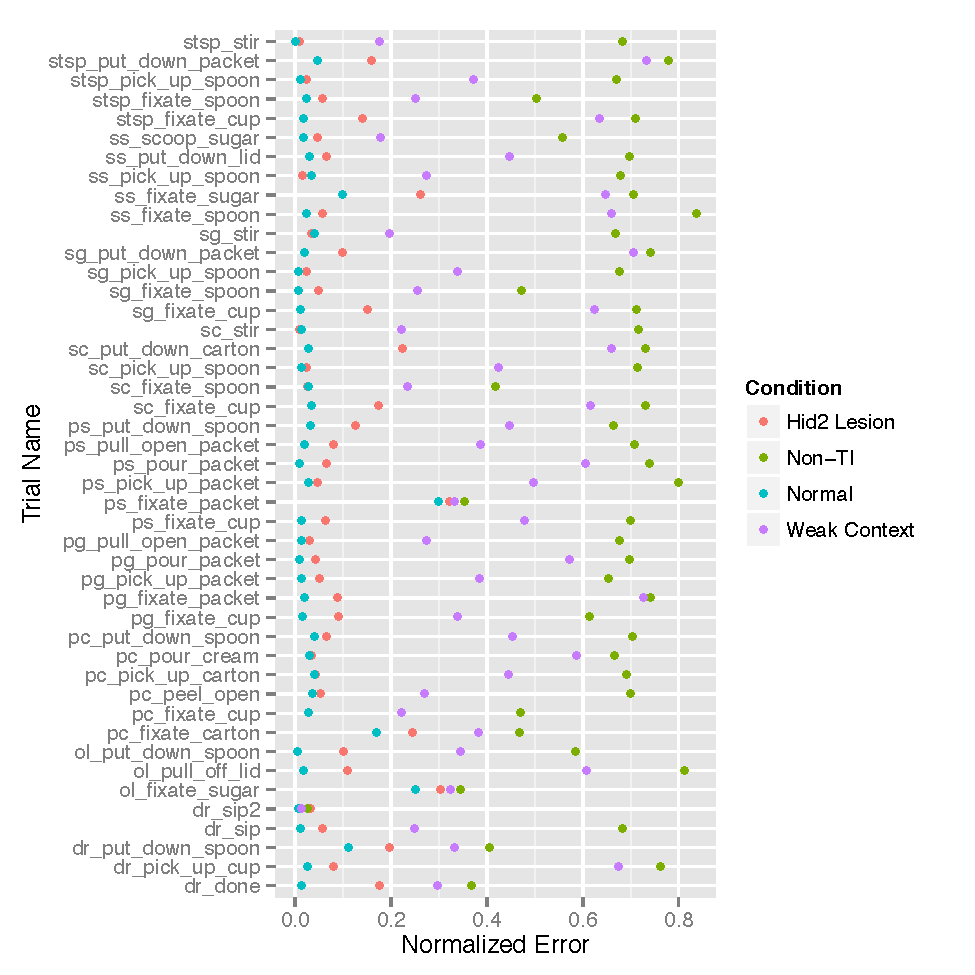
\includegraphics[width=\textwidth]{figs/test_error}
  \caption{Normalized error for each test trial is shown for different manipulations of 100 trained networks. The Normal (2 hidden layers with 24 units) network structure performs the best, but shows some error for the ol\_fixate\_sugar and ps\_fixate\_packet trials. The Non-TI version performs the worst for every trial type. Even the Weak Context performs somewhat better (with great variability--some steps are near-normal, while others are close to Non-TI error rates). Finally, lesioning the second hidden layer (Hid2 Lesion) only moderately decreases performance.}
  \label{fig:test_error}
\end{figure}


\clearpage
%%%%%%%%%%%%%%%%%%%%%%%%%%%%%%%%%%%%%%%%%%%%%%%%%%%%%%%%%%%

\bibliographystyle{apacitex} % apalike / apacite
\bibliography{tec_references}
%\printbibliography


% Footer
\begin{center}
  \begin{footnotesize}
    Last updated: \today 
  \end{footnotesize}
\end{center}

\end{document}